\documentclass{article}

\usepackage[utf8]{inputenc}
\usepackage[T1]{fontenc}

\usepackage{geometry}
 \geometry{
 a4paper,
 total={170mm,257mm},
 left=20mm,
 top=20mm,
 }

\setlength{\parskip}{7pt}
\setlength{\parindent}{0pt}

\title{OpenOCD for RISC-V}
\date{2019-10-14}

\PassOptionsToPackage{hyphens}{url}\usepackage{hyperref}
\usepackage{listings}
\usepackage{amssymb}
\usepackage{graphicx}
\graphicspath{ {./images/} }
\usepackage{float}

\lstset{
	breaklines=true,
	columns=fullflexible,
	tabsize=4,
	showstringspaces=false,
	frame=single
}

\begin{document}
	\maketitle
	
	\section{About}
	
	OpenOCD is a software that provides on-chip debugging, in-system programming and boundary-scan testing tools.
	
	The official website is \url{openocd.org}
	
	\begin{figure}[H]
	\centering
	
\includegraphics[width=0.6\textwidth]{openocd.png}
	\end{figure}
	
	A fork with RISC-V support is available on \url{https://github.com/riscv/riscv-openocd}
	
	OpenOCD is free software and is licensed under the \textbf{GNU General Public License v2.0}
	
	This document presents a way of using OpenOCD to debug a RISC-V platform using a JTAG connection.
	
	
	\newpage
	\section{Position in the debug system}
	
	OpenOCD can be used as a translator between GDB and a RISC-V platform, as can be seen in the RISC-V external debug specification.
	
	\begin{figure}[H]
   	\centering
   	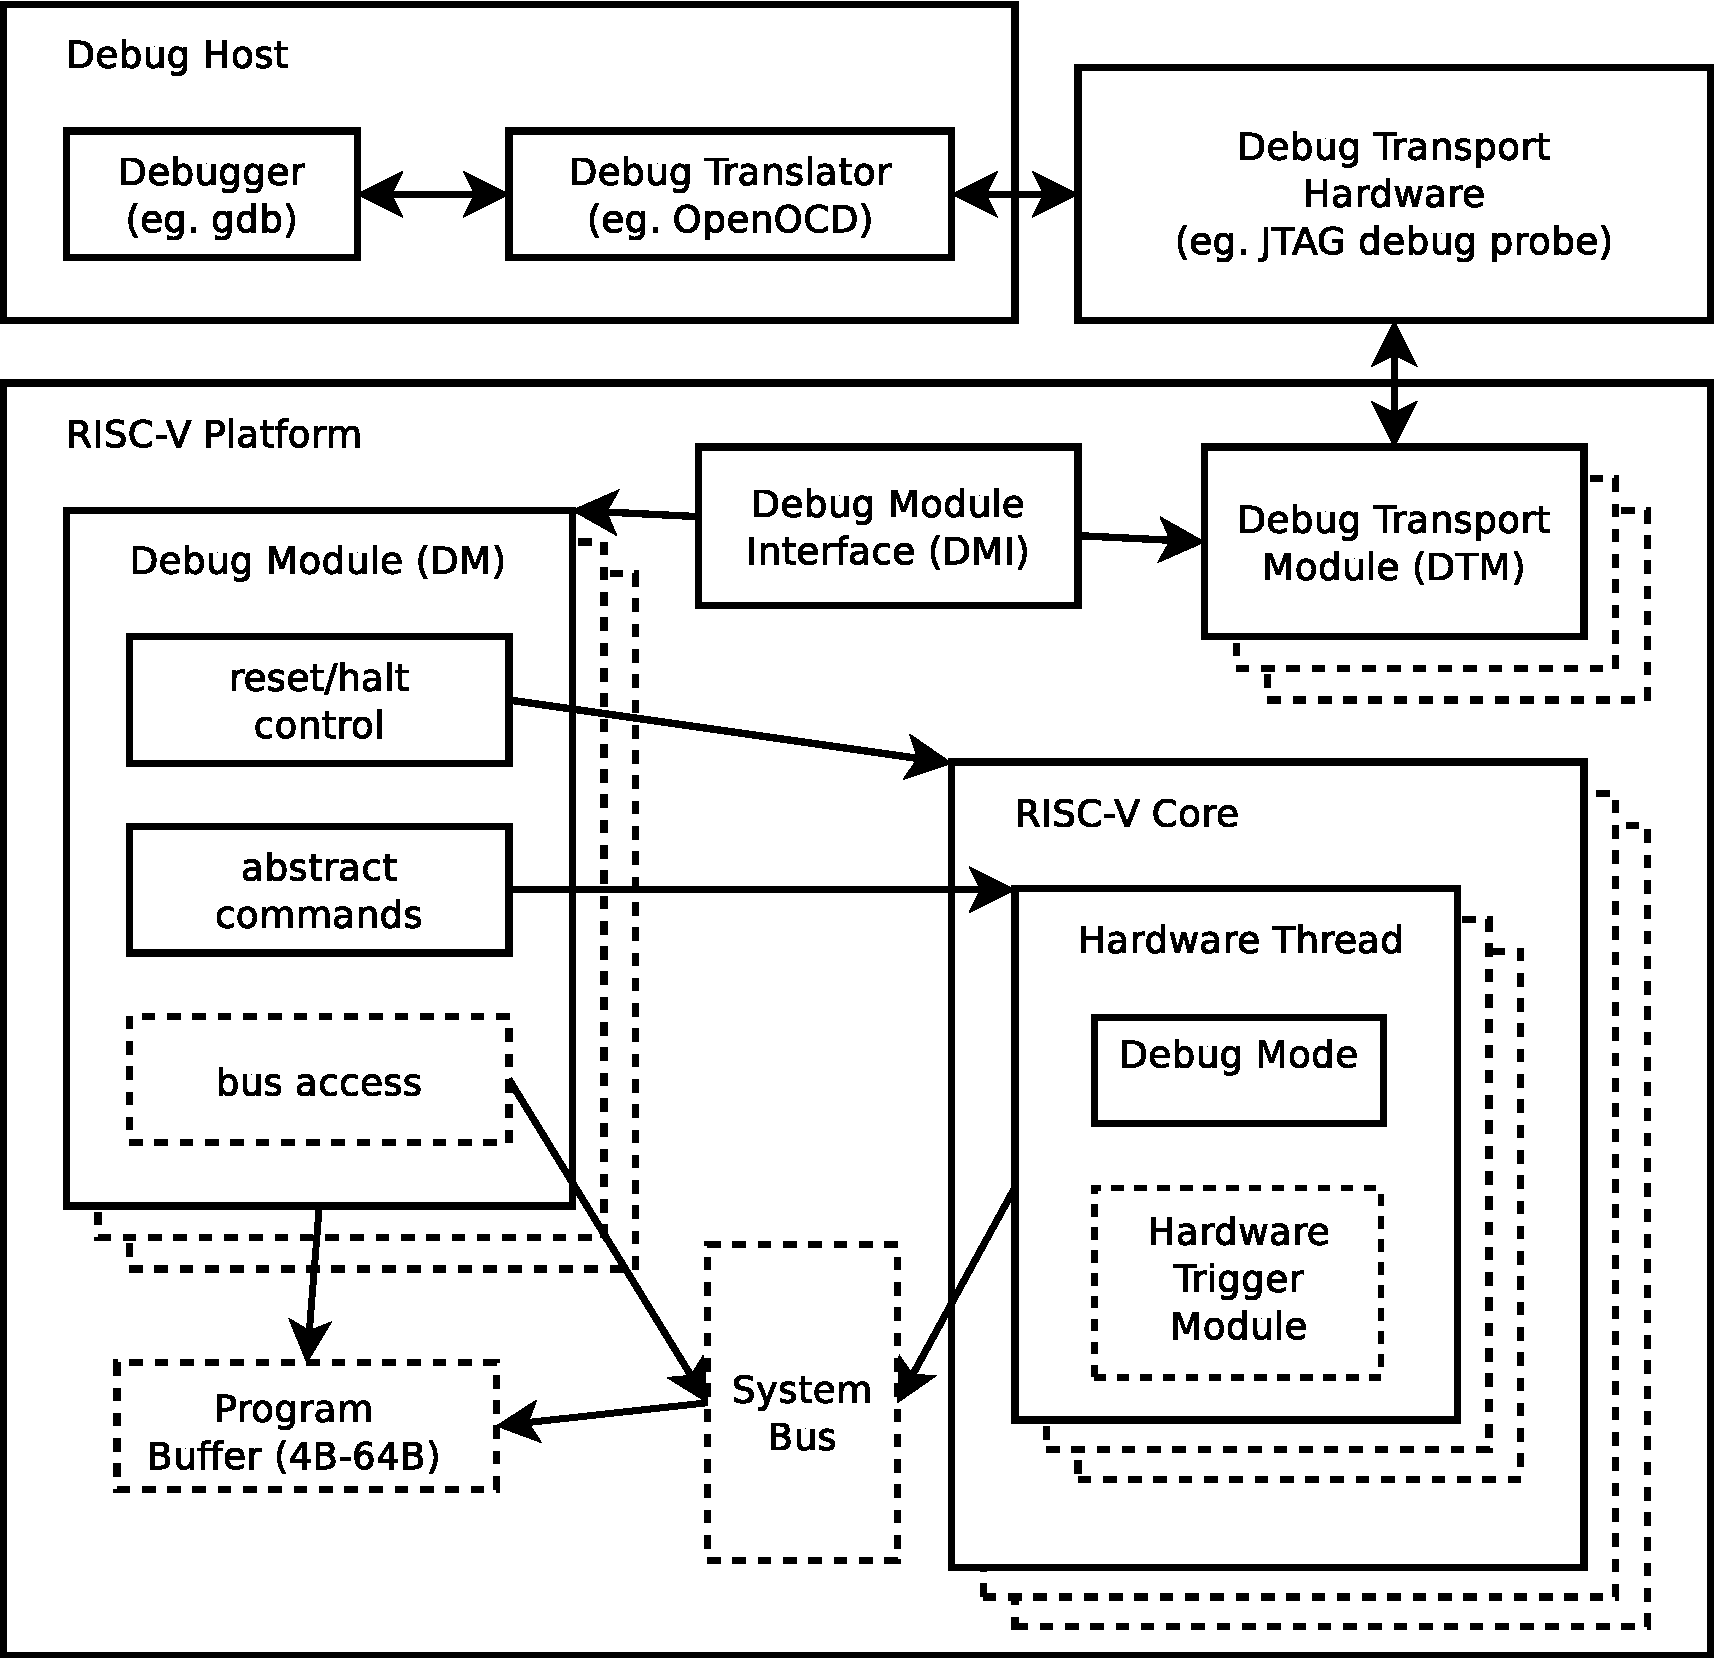
\includegraphics[width=0.82\textwidth]{overview.pdf}
   	\caption{RISC-V Debug System Overview}
   	\label{fig:overview}
	\end{figure}
	
	OpenOCD can connect to GDB in two ways: with a TCP/IP socket or with pipes (stdin/stdout). 
	
	More information here: \url{http://openocd.org/doc-release/html/GDB-and-OpenOCD.html}
	
	A debug adapter is needed to connect OpenOCD to the RISC-V platform. This document focuses on using JTAG transport hardware.
	
	\newpage
	\section{Config file}
	
	\url{http://openocd.org/doc-release/html/OpenOCD-Project-Setup.html}
	
	A typical usage of OpenOCD is:
	
	\begin{lstlisting}[language=bash]
    $ openocd -f config_file.cfg
    \end{lstlisting}
    
    A config file contains commands that OpenOCD will execute using its Jim-Tcl interpreter.
    
    A single file can be broken into several ones. The command line call would then list every file in the correct order:
    
    \begin{lstlisting}[language=bash]
    $ openocd -f config_file_1.cfg config_file_2.cfg config_file_3.cfg
    \end{lstlisting}
    
    It is also possible to launch a single command:
    
    \begin{lstlisting}[language=bash]
    $ openocd -c "a command"
    \end{lstlisting}
    
    To have more information about what OpenOCD is doing, use the -d option.
    
    \begin{lstlisting}[language=bash]
    $ openocd -f config_file.cfg -d
    \end{lstlisting}
    
    \subsection{Interface}
    
    \url{http://openocd.org/doc-release/html/Debug-Adapter-Configuration.html}
    
    The interface configuration tells OpenOCD how to use the transport hardware. 
    
    Config files for a lot of debug adapters can be found where OpenOCD was installed. The path should be \textbf{<build>/share/openocd/scripts/interface}.
    
    Otherwise, refer to examples and the official documentation to see how to use the various interface drivers.
    
    \subsection{TAP declaration}
    
    \url{http://openocd.org/doc-release/html/TAP-Declaration.html}
    
    A device with a JTAG interface means the device has a Test Access Port (TAP). You need to set up the active TAPs of the device by declaring them inside a configuration file.
    
    Typically, this is achieved in a few lines:
    
    \begin{lstlisting}[language=tcl]
    set _CHIPNAME riscv
    jtag newtap $_CHIPNAME cpu -irlen 5 -expected-id 0x12345678
    \end{lstlisting}
    
    The -irlen parameter is the length in bits of the TAP instruction register and is mandatory.
    
    You can give the IDCODE which is expected in the TAP, but this is optionnal.
    
    \subsection{CPU configuration}
    
    \url{http://openocd.org/doc-release/html/CPU-Configuration.htm}
    
    This step gives information about the debug target.
    
    \begin{lstlisting}[language=tcl]
    set _TARGETNAME $_CHIPNAME.cpu
    target create $_TARGETNAME riscv -chain-position $_TARGETNAME
    \end{lstlisting}
    
    The target refers to a TAP with a \textit{dotted.name} and its type is precised (riscv for RISC-V).
    
    \subsection{Starting the debug session}
    
    \url{http://openocd.org/doc/html/Server-Configuration.html}
    
    \url{http://openocd.org/doc-release/html/General-Commands.html}
    
    An end of the config file could be:
    
    \begin{lstlisting}[language=tcl]
    init
    halt
    \end{lstlisting}
    
    \textbf{init} end the configuration stages and enters the run stage.
    
    \textbf{halt} sends a halt request to the target.
    
    Afetr these commands, the target is halted and OpenOCD is waiting for a GDB connection.
    
    \subsection{Other useful commands}
    
    \url{http://openocd.org/doc/html/index.html}
    
    All commands are detailed in the official documentation. From experience, the following commands have been useful.
    
    Set up a maximum speed for the JTAG interface:
    
    \begin{lstlisting}[language=tcl]
    adapter_khz 1000
    \end{lstlisting}
    
    Enable error reports from GDB:
    
    \begin{lstlisting}[language=tcl]
    gdb_report_data_abort enable
    gdb_report_register_access_error enable
    \end{lstlisting}
    
    Display the TAPs in the scan chain and their status:
    
    \begin{lstlisting}[language=tcl]
    scan_chain
    \end{lstlisting}
    
    Prefer to use the System Bus Access to access memory rather than the Program Buffer:
    
    \begin{lstlisting}[language=tcl]
    riscv set_prefer_sba on
    \end{lstlisting}
    
    By default, OpenOCD will only listen on the loopback network interface (localhost). If the network environment is safe, you can cover all available interfaces with:
    
    \begin{lstlisting}[language=tcl]
    bindto 0.0.0.0
    \end{lstlisting}
    
    \newpage
    \section{Config file examples}
    
    \subsection{remote\_bitbang interface}
    
    \url{https://github.com/riscv/riscv-isa-sim#debugging-with-gdb}
    
    The RISC-V ISA simulator Spike can be interfaced with OpenOCD and GDB. The corresponding config file is given in the project \textit{README.md}
    
    \begin{lstlisting}[language=tcl]
interface remote_bitbang
remote_bitbang_host localhost
remote_bitbang_port 9824

set _CHIPNAME riscv
jtag newtap $_CHIPNAME cpu -irlen 5 -expected-id 0x10e31913

set _TARGETNAME $_CHIPNAME.cpu
target create $_TARGETNAME riscv -chain-position $_TARGETNAME

gdb_report_data_abort enable

init
halt
    \end{lstlisting}
    
    The interface driver is \textbf{remote\_bitbang}. It connects to a remote process over a socket connection and performs bitbang requests. This driver is useful for debugging a simulated processor.
    
    You need to specify a port number and a hostname to the driver.
    
    \subsection{sysfsgpio interface}
    
    \url{http://openocd.org/doc/doxygen/html/sysfsgpio_8c.html#details}
    
    The \textbf{sysfsgpio} interface driver implements a bitbang JTAG interface using system GPIOs.
    
    \begin{lstlisting}[language=tcl]
adapter_khz		10000

interface sysfsgpio

# gpio numbers: tck tms tdi tdo
sysfsgpio_jtag_nums 507 508 509 510

# gpio number: trst
sysfsgpio_trst_num 511 

set _CHIPNAME riscv
jtag newtap $_CHIPNAME cpu -irlen 5

set _TARGETNAME $_CHIPNAME.cpu
target create $_TARGETNAME riscv -chain-position $_TARGETNAME

gdb_report_data_abort enable
bindto 0.0.0.0

init
halt
    \end{lstlisting}
    
    \newpage
    \subsection{ftdi interface and several TAPs}
    
    \url{https://github.com/pulp-platform/pulpissimo}
    
    The pulpissimo project provides several examples of using the \textbf{ftdi} interface driver and setting up a scan chain with two TAPs.
      
    An example for the Olimex ARM-USB-OCD debug adapater is:
    
    \begin{lstlisting}[language=tcl]

adapter_khz     1000

# Olimex ARM-USB-OCD-H
interface ftdi
ftdi_device_desc "Olimex OpenOCD JTAG ARM-USB-OCD-H"
ftdi_vid_pid 0x15ba 0x002b

ftdi_layout_init 0x0908 0x0b1b
ftdi_layout_signal nSRST -oe 0x0200
ftdi_layout_signal nTRST -data 0x0100
ftdi_layout_signal LED -data 0x0800


set _CHIPNAME riscv

jtag newtap $_CHIPNAME unknown0 -irlen 5 -expected-id 0x10102001
jtag newtap $_CHIPNAME cpu -irlen 5 -expected-id 0x249511C3

set _TARGETNAME $_CHIPNAME.cpu
target create $_TARGETNAME riscv -chain-position $_TARGETNAME -coreid 0x3e0

gdb_report_data_abort enable
gdb_report_register_access_error enable

riscv set_reset_timeout_sec 120
riscv set_command_timeout_sec 120

# prefer to use sba for system bus access
riscv set_prefer_sba on

# dump jtag chain
scan_chain


init
halt
echo "Ready for Remote Connections"
    \end{lstlisting}
    
    The interface part of the configuration can also be found in the scripts provided by OpenOCD in your build directory: \textbf{<build>/share/openocd/scripts/interface/ftdi/olimex-arm-usb-ocd.cfg}
    
    There are two TAPs in the scan chain, but only one is compatible with OpenOCD. Both are described in the config file, but only one is linked with a target.
    
	
\end{document}